\documentclass[14pt]{extarticle}

\usepackage{fontspec}
\setmainfont{Times New Roman}

% размер полей
\usepackage{geometry}
\geometry{a4paper, top=2cm, bottom=2cm, right=1.5cm, left=3cm}

 %debugging
%\usepackage{showframe}

% полуторный интервал
\usepackage{setspace}
\onehalfspacing

% абзацный отступ
\setlength{\parindent}{1.25cm}

% выравнивание текста по ширине
\sloppy

% списки
\usepackage{calc} % арифметические операции с величинами
\usepackage{enumitem}
\setlist{
    nosep,
    leftmargin=0pt,
    itemindent=\parindent + \labelwidth - \labelsep,
}

% подписи к рисункам и таблицам
\usepackage{caption}
\renewcommand{\figurename}{Рисунок}
\renewcommand{\tablename}{Таблица}
\DeclareCaptionFormat{custom}
{
    \textit{#1#2#3}
}
\DeclareCaptionLabelSeparator{custom}{. }
\captionsetup{
    % хз какой это размер - 12 или нет, но выглядит меньше 14
    font=small,
    format=custom,
    labelsep=custom,
}

% картинки
\usepackage{graphicx}

% колонтитулы
\usepackage{fancyhdr}

% картинки и таблицы находятся именно в том месте текста где помещены (атрибут H)
\usepackage{float}

% таблицы
\usepackage{tabularray}

\graphicspath{ {5.2.1/models/} }
\begin{document}
\pagestyle{fancy}
\fancyhead{}
% disable header
\renewcommand{\headrulewidth}{0pt}
\fancyfoot[L]{Дубровских гр 221-361}
\fancyfoot[C]{ЛР 5.2.1}
\fancyfoot[R]{Продажа автотранспорта}
\singlespacing

\newpage
\begin{center}
    Министерство науки и высшего образования Российской Федерации
    Федеральное государственное автономное образовательное учреждение

    высшего образования

    \guillemotleft МОСКОВСКИЙ ПОЛИТЕХНИЧЕСКИЙ УНИВЕРСИТЕТ\guillemotright

    (МОСКОВСКИЙ ПОЛИТЕХ)
\end{center}
\noindent
\bigbreak
\bigbreak
\bigbreak
\bigbreak
\begin{center}
    ЛАБОРАТОРНАЯ РАБОТА 5.2.1

    По курсу Проектирования пользовательских интерфейсов в веб

    \textbf{Проектирование композиции и визуальной иерархии в макете веб-страниц и мобильного устройства}
    \bigbreak
    \bigbreak
    \bigbreak
    \bigbreak
    ТЕМА

    \guillemotleft\textbf{САЙТ ДЛЯ ПРОДАЖИ И ПОИСКА АВТОМОБИЛЕЙ}\guillemotright
\end{center}
\noindent
\bigbreak
\bigbreak
\bigbreak
\bigbreak
\bigbreak
\bigbreak
\bigbreak
\bigbreak
\bigbreak
\bigbreak
\hfill Выполнил

\hfill Дубровских Никита Евгеньевич

\hfill Группа 221-361
\bigbreak
\bigbreak
\bigbreak
\hfill Проверил

\hfill Натур ВВ
\vfill
\begin{center}
    Москва, 2024
\end{center}
\newpage
\onehalfspacing


\begin{center}
    \textbf{Лабораторная работа 5.2.1}

    \textbf{Проектирование композиции и визуальной иерархии в макете веб-страниц и мобильного устройства}
\end{center}

\textbf{Цель работы:} композиционно выстроить основные элементы интерфейса главной страницы веб-сайта
\bigskip

\textbf{Задачи:}

\begin{enumerate}
    \item Изучить основы построения композиции
    \item Выстроить элементы интерфейса главной страницы согласно принципам визуальной иерархии
    \item Выстроить элементы интерфейса главной страницы согласно «правилу третей» и правилу «золотого сечения», паттернам сканирования
\end{enumerate}
\bigskip

\textbf{Основные термины}

\begin{itemize}
    \item Композиция - организация элементов дизайна, обеспечивающая гармоничное и логичное восприятие целого.
    \item Принципы композиции - включают целесообразность, единство и соподчиненность, равновесие, наличие смыслового центра, гармонию.
    \item Правило третей - метод зонирования страницы с делением на три части, где основные элементы располагаются на пересечениях линий для привлечения внимания.
    \item Золотое сечение - пропорция, создающая гармоничное восприятие элементов интерфейса, часто используется для зонирования и распределения элементов.
    \item Золотая спираль (спираль Фибоначчи) - инструмент для размещения элементов от меньших к большим по мере увеличения витков спирали.
    \item Паттерны сканирования (айтрекинг) - наблюдение за движением взгляда пользователя по сайту для оптимизации навигации.
    \item Диаграмма Гутенберга - схема восприятия, где внимание пользователя концентрируется на ключевых зонах страницы.
    \item Визуальная иерархия - структурирование элементов интерфейса для правильного восприятия пользователем, с фокусом на главные элементы.
    \item Фокальная точка - основной элемент композиции, привлекающий внимание.
    \item Баланс и пропорции - равновесие и соразмерность элементов, обеспечивающие устойчивость и гармонию.
    \item Контраст - различие свойств элементов, подчеркивающее их значимость и создающее интерес.
    \item Цветовая гармония - использование цветов для создания целостного и сбалансированного дизайна.
    \item Типографика - выбор и размещение текста для создания иерархии и привлечения внимания.
    \item Пространство - использование пустого места для выделения важных элементов и создания баланса.
    \item Айтрекинг - технология для отслеживания движения взгляда по интерфейсу, помогает оптимизировать расположение элементов.
\end{itemize}
\bigskip

\textbf{Страницы сайтов с приёмами композиции}
\bigskip

\noindent
\begin{minipage}{\linewidth}
    \fbox{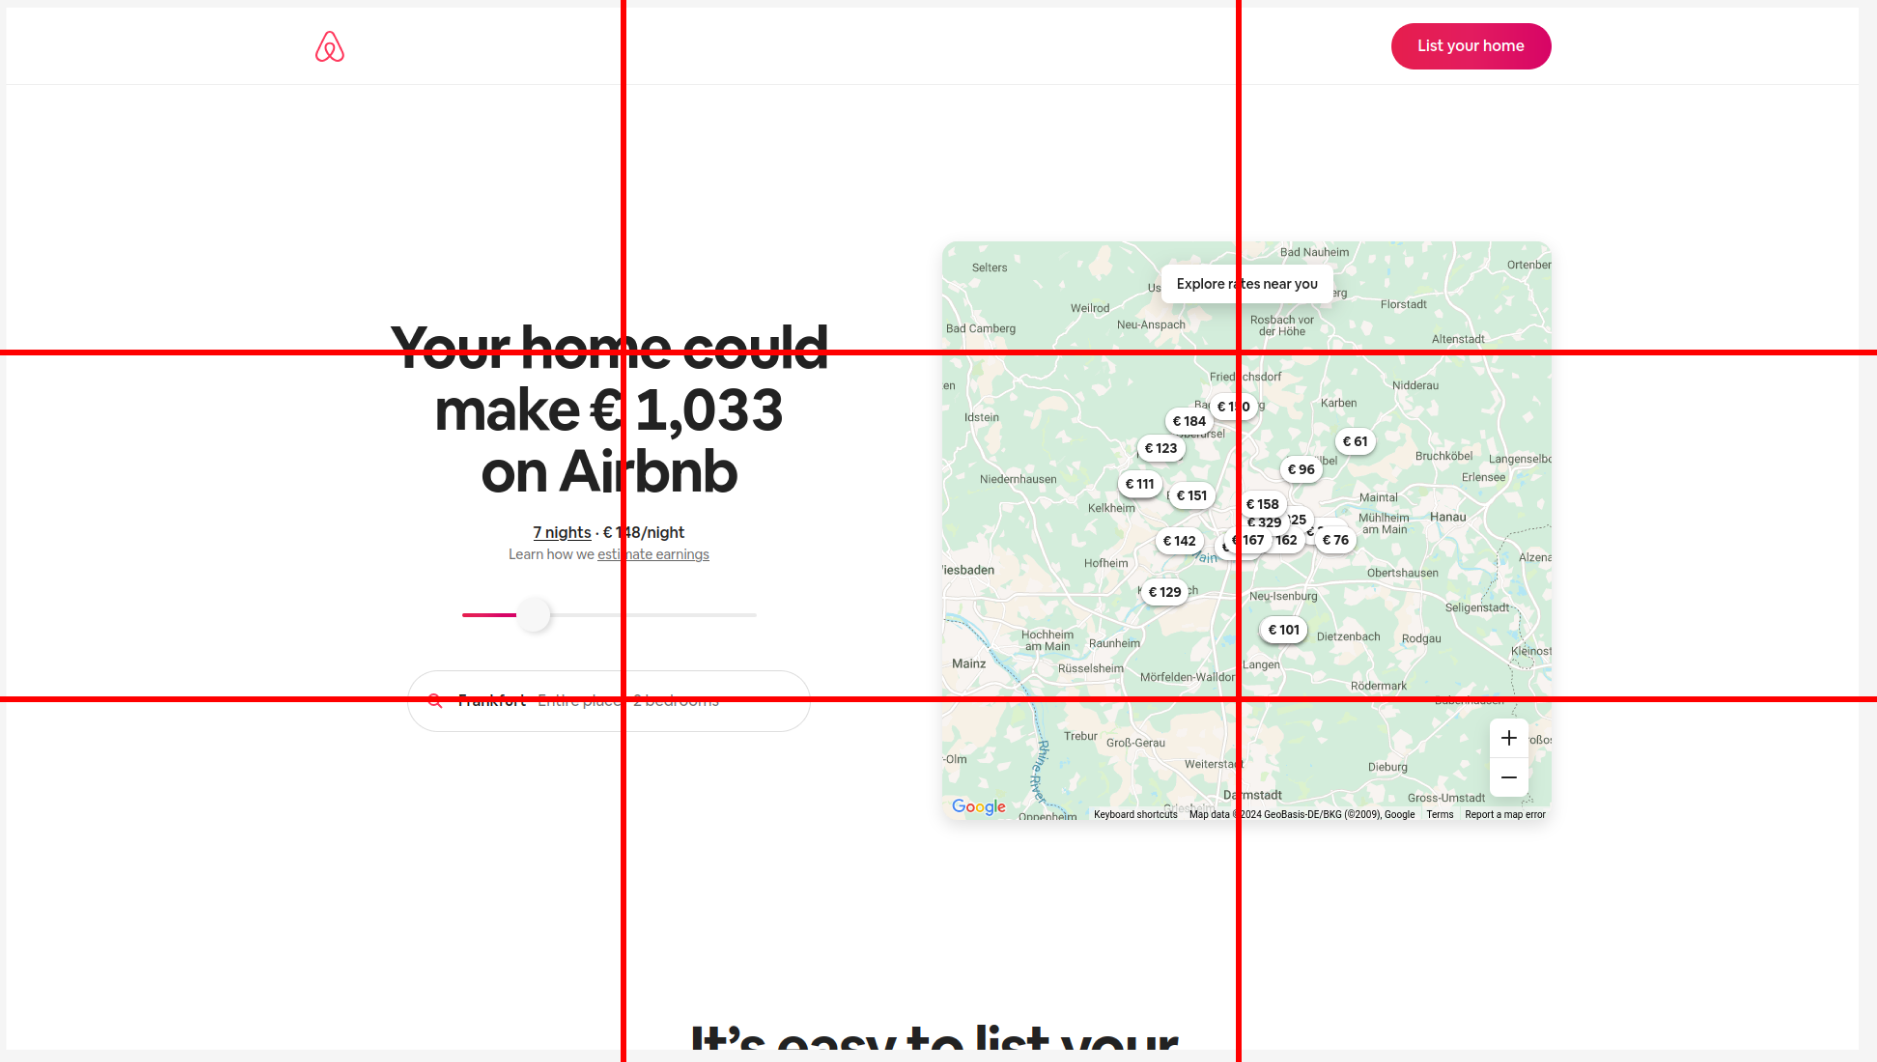
\includegraphics[width=\linewidth]{airbnb_thirds}}
    \captionof{figure}{Правило третей на сайте airbnb.com/host/homes}
\end{minipage}
\bigskip

\noindent
\begin{minipage}{\linewidth}
    \fbox{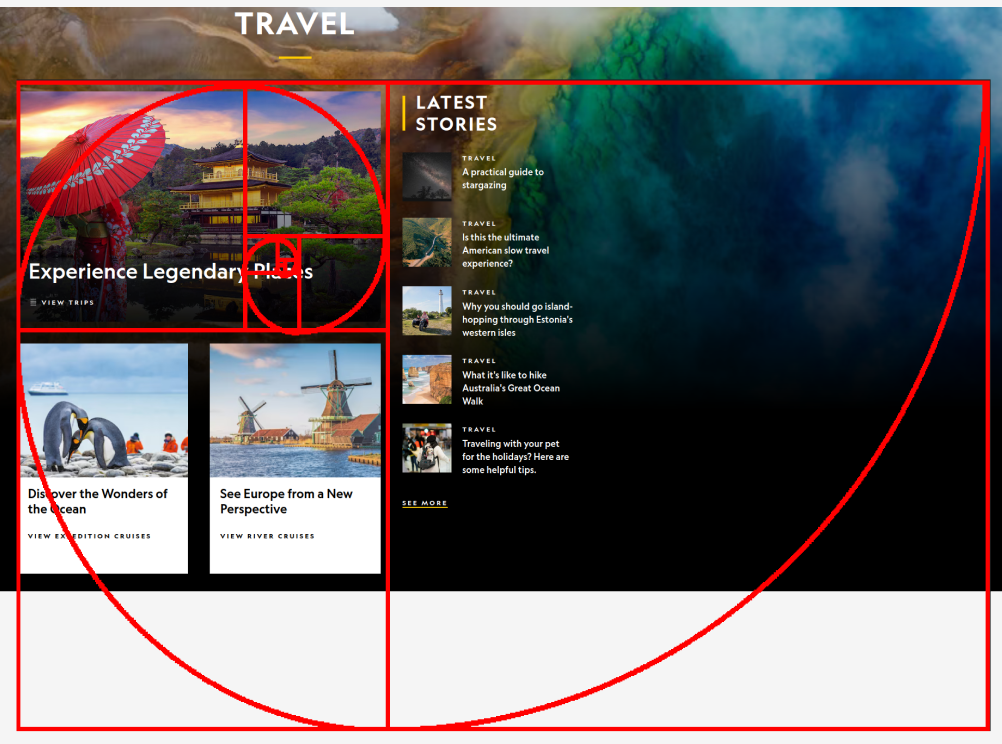
\includegraphics[width=\linewidth]{ng_spiral}}
    \captionof{figure}{Золотая спираль Фибоначчи на сайте nationalgeographic.com}
\end{minipage}
\bigskip

\noindent
\begin{minipage}{\linewidth}
    \fbox{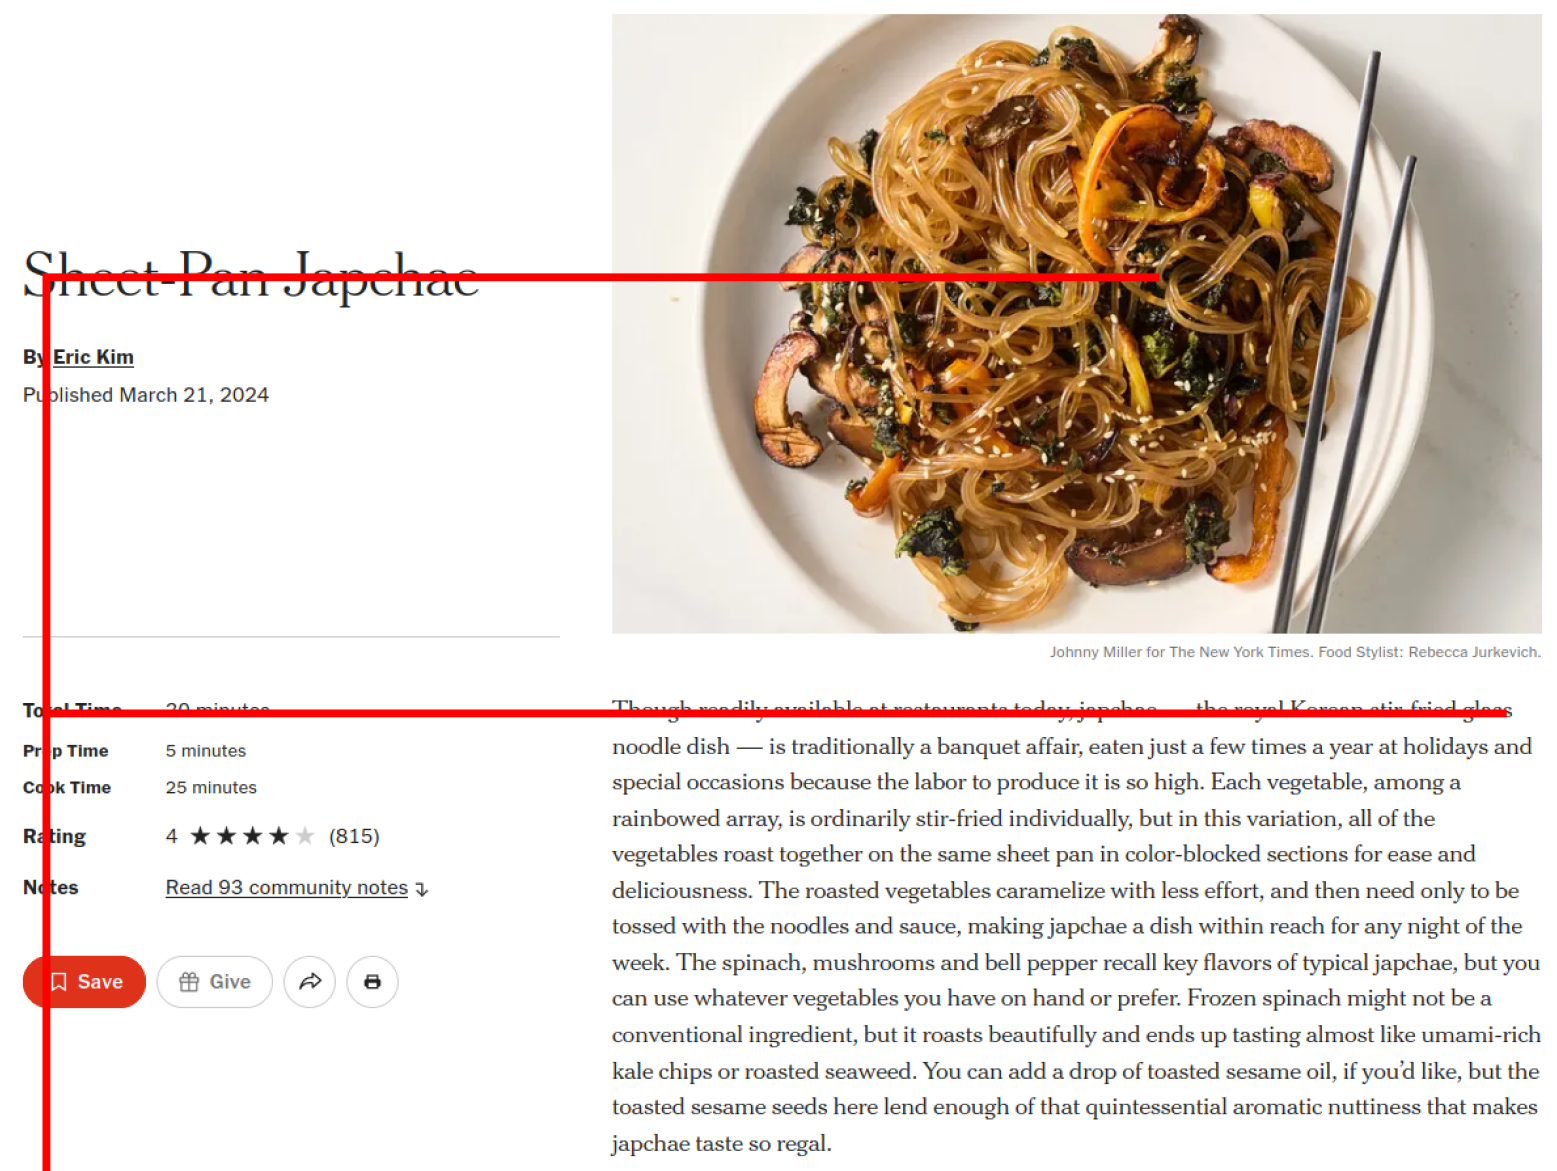
\includegraphics[width=\linewidth]{nytimes_f}}
    \captionof{figure}{F-паттерн на сайте cooking.nytimes.com/recipes/1025197-sheet-pan-japchae}
\end{minipage}
\bigskip

\noindent
\begin{minipage}{\linewidth}
    \fbox{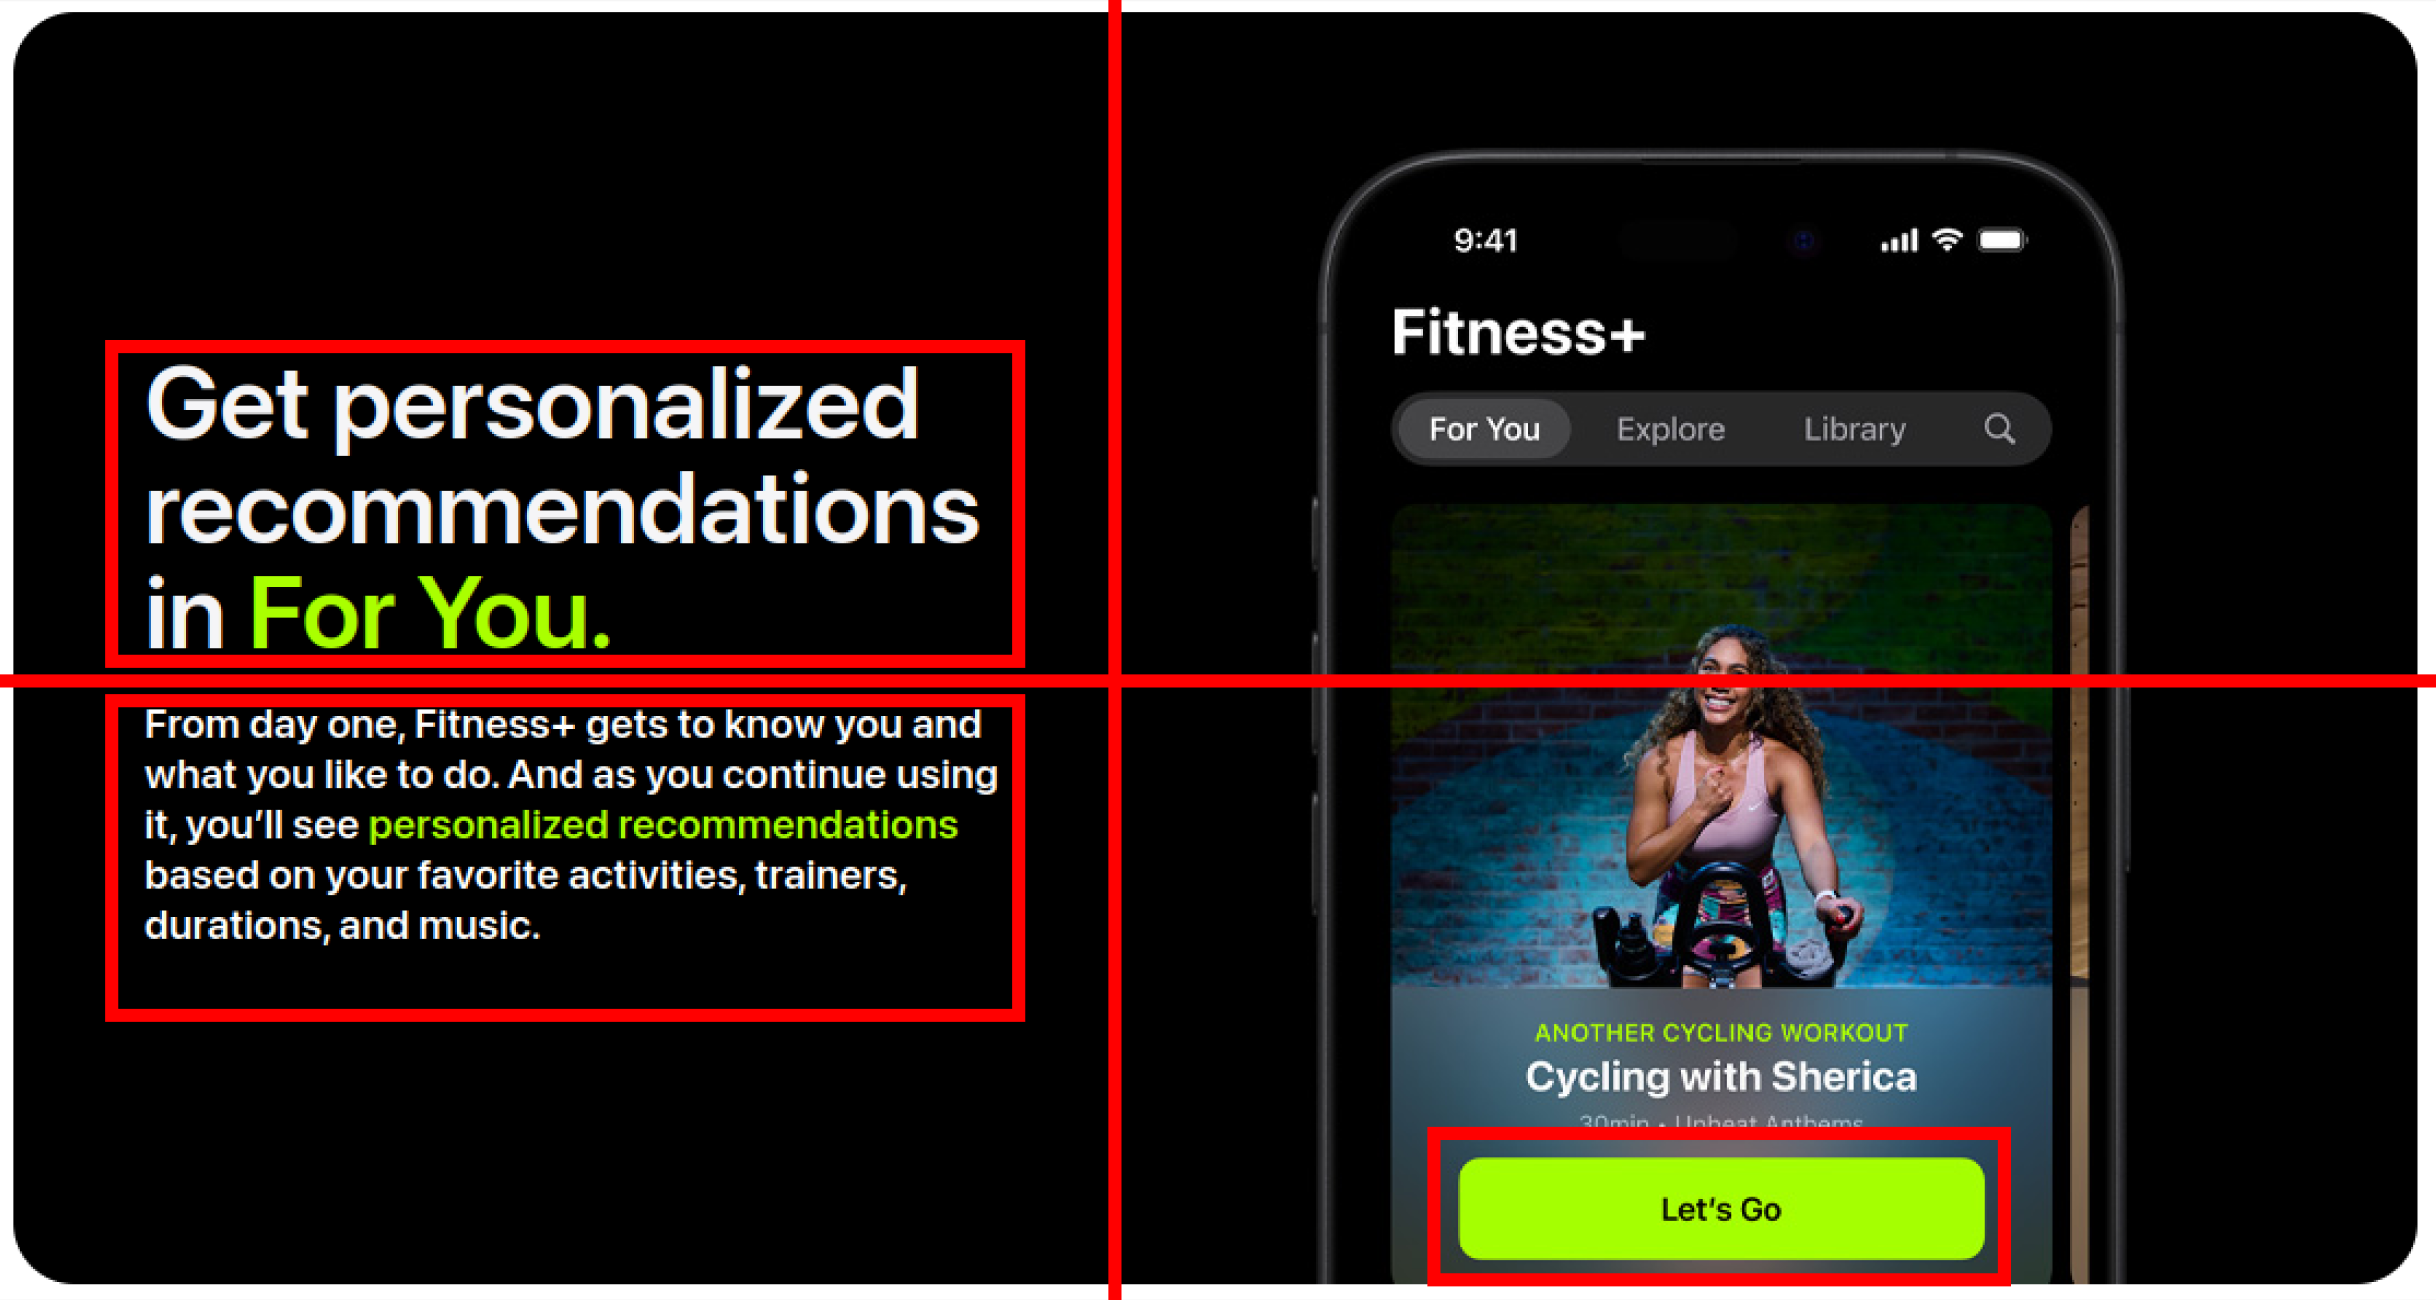
\includegraphics[width=\linewidth]{apple_diag}}
    \captionof{figure}{Диаграмма Гутенберга на сайте apple.com/apple-fitness-plus}
\end{minipage}
\bigskip

\noindent
\begin{minipage}{\linewidth}
    \fbox{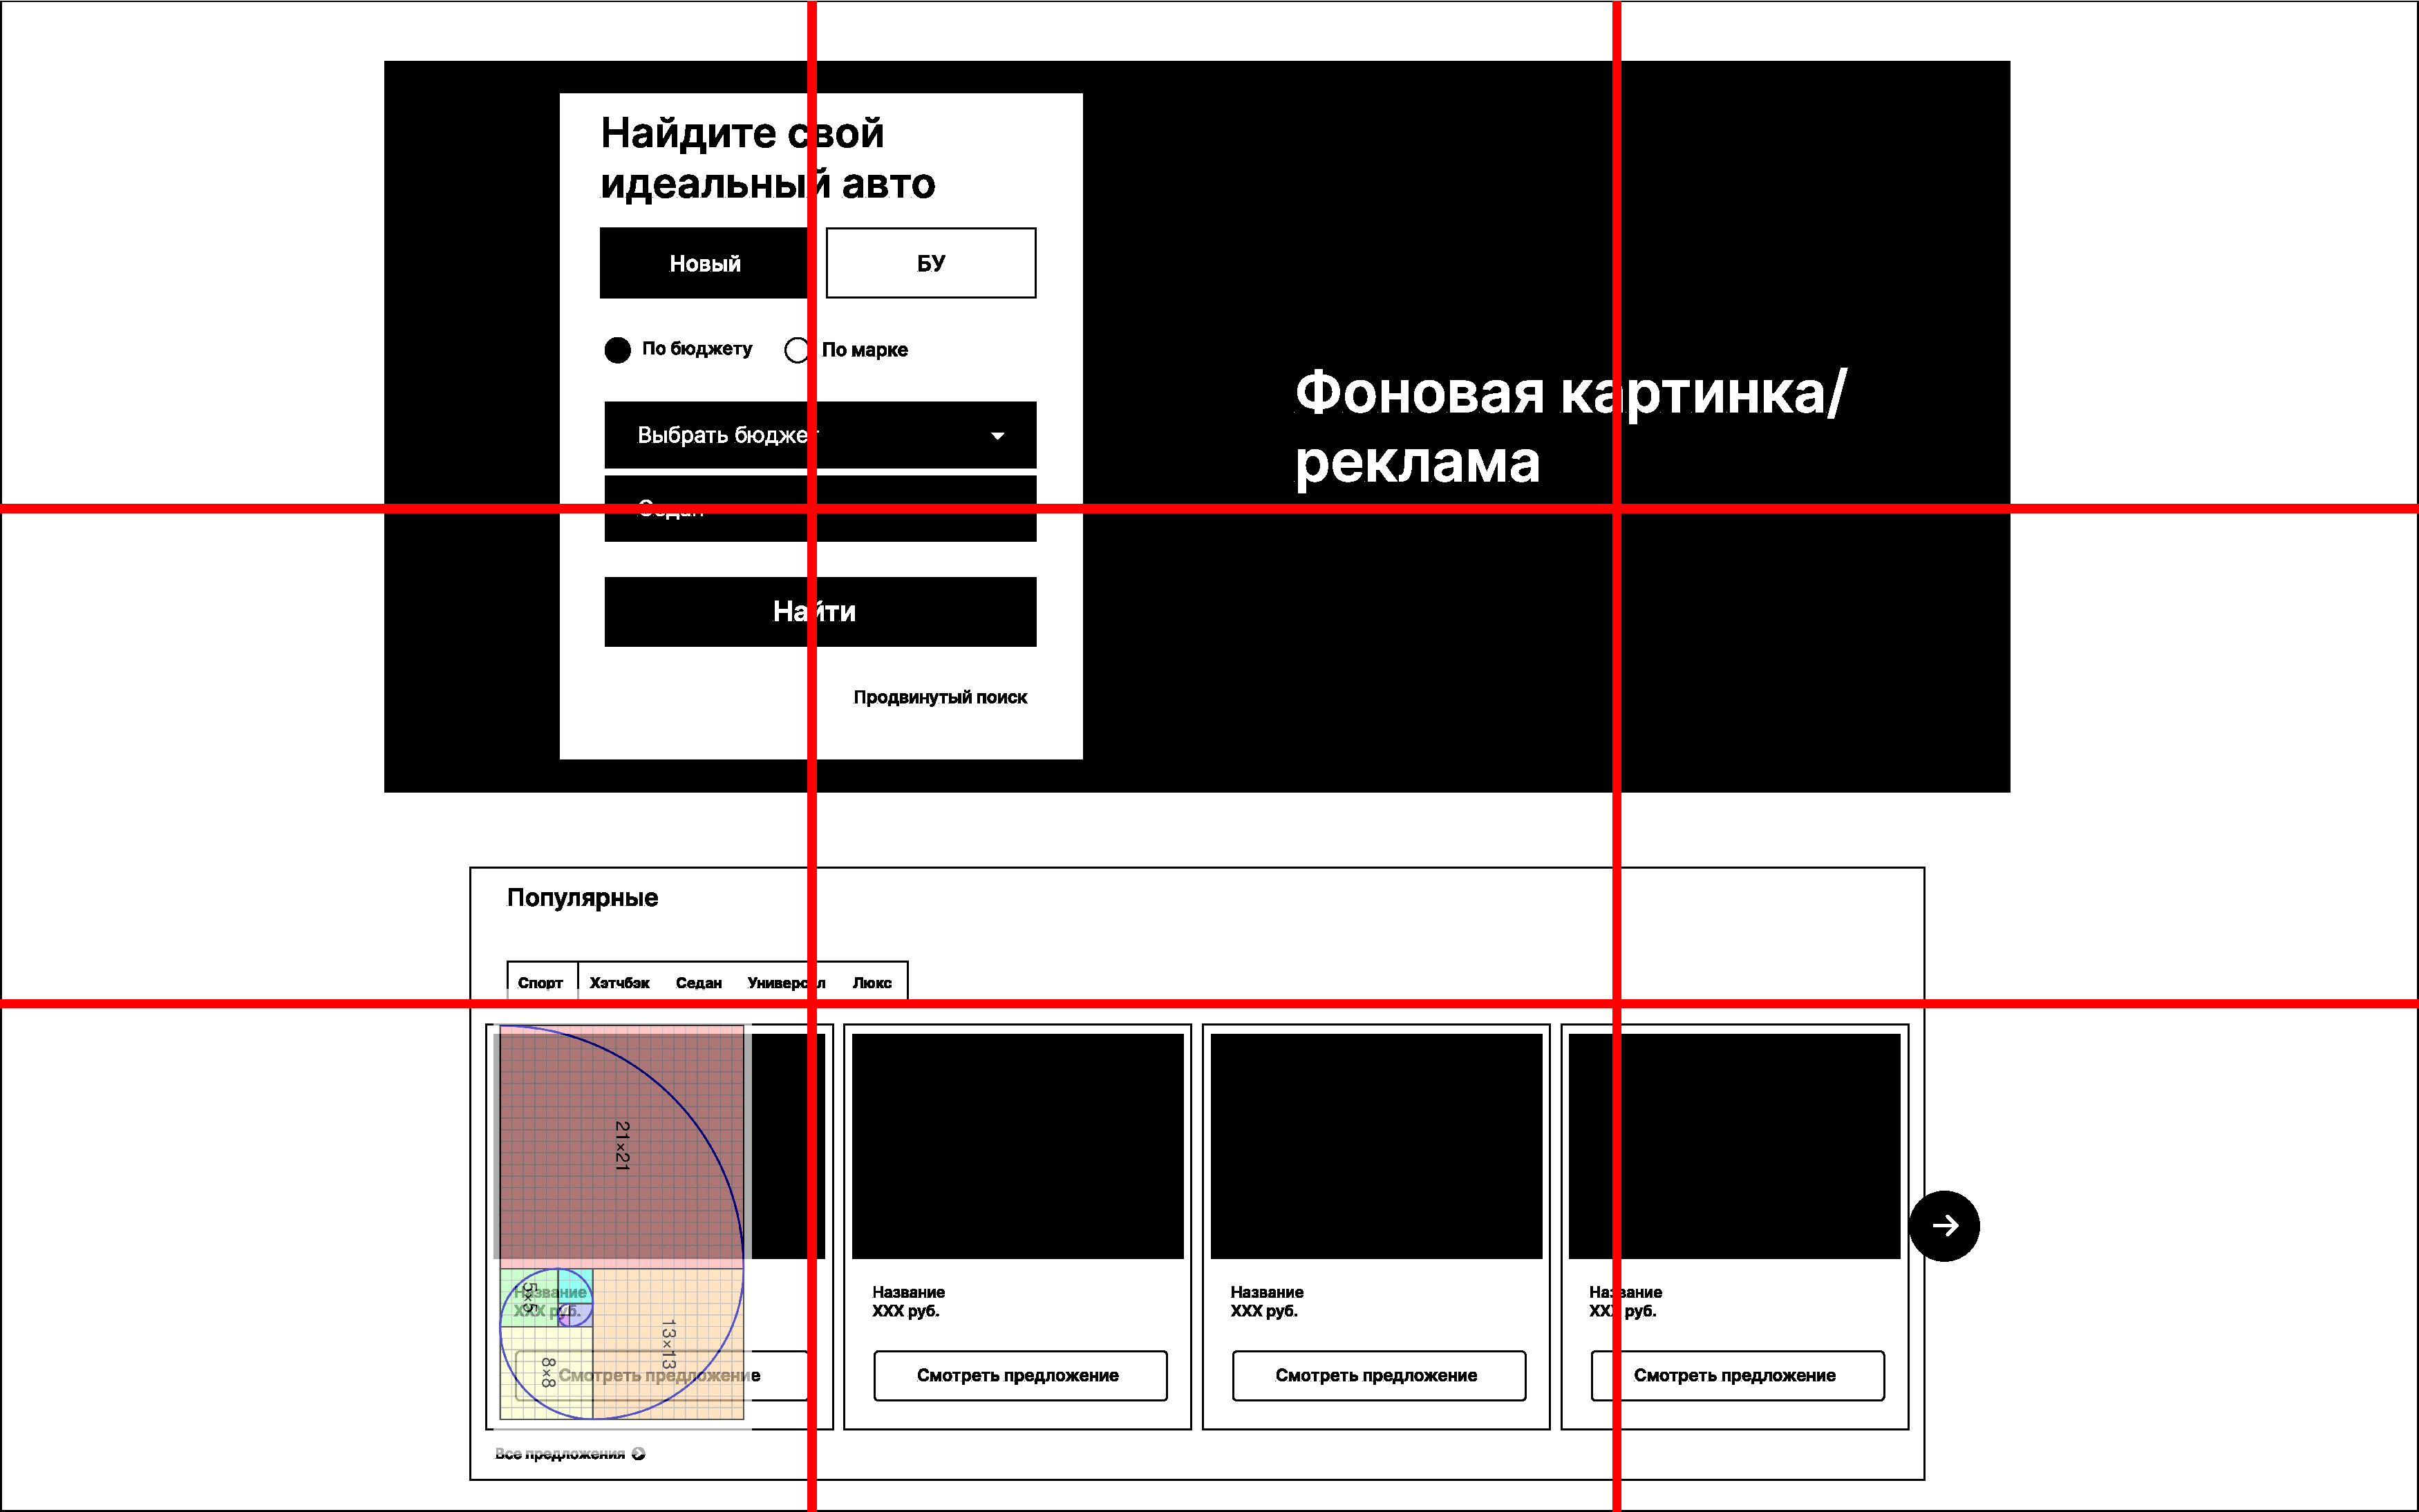
\includegraphics[width=\linewidth]{Main_comp}}
    \captionof{figure}{Правило третей и золотая спирать Фибоначчи на главной странице}
\end{minipage}
\bigskip

\noindent
\begin{minipage}{\linewidth}
    \fbox{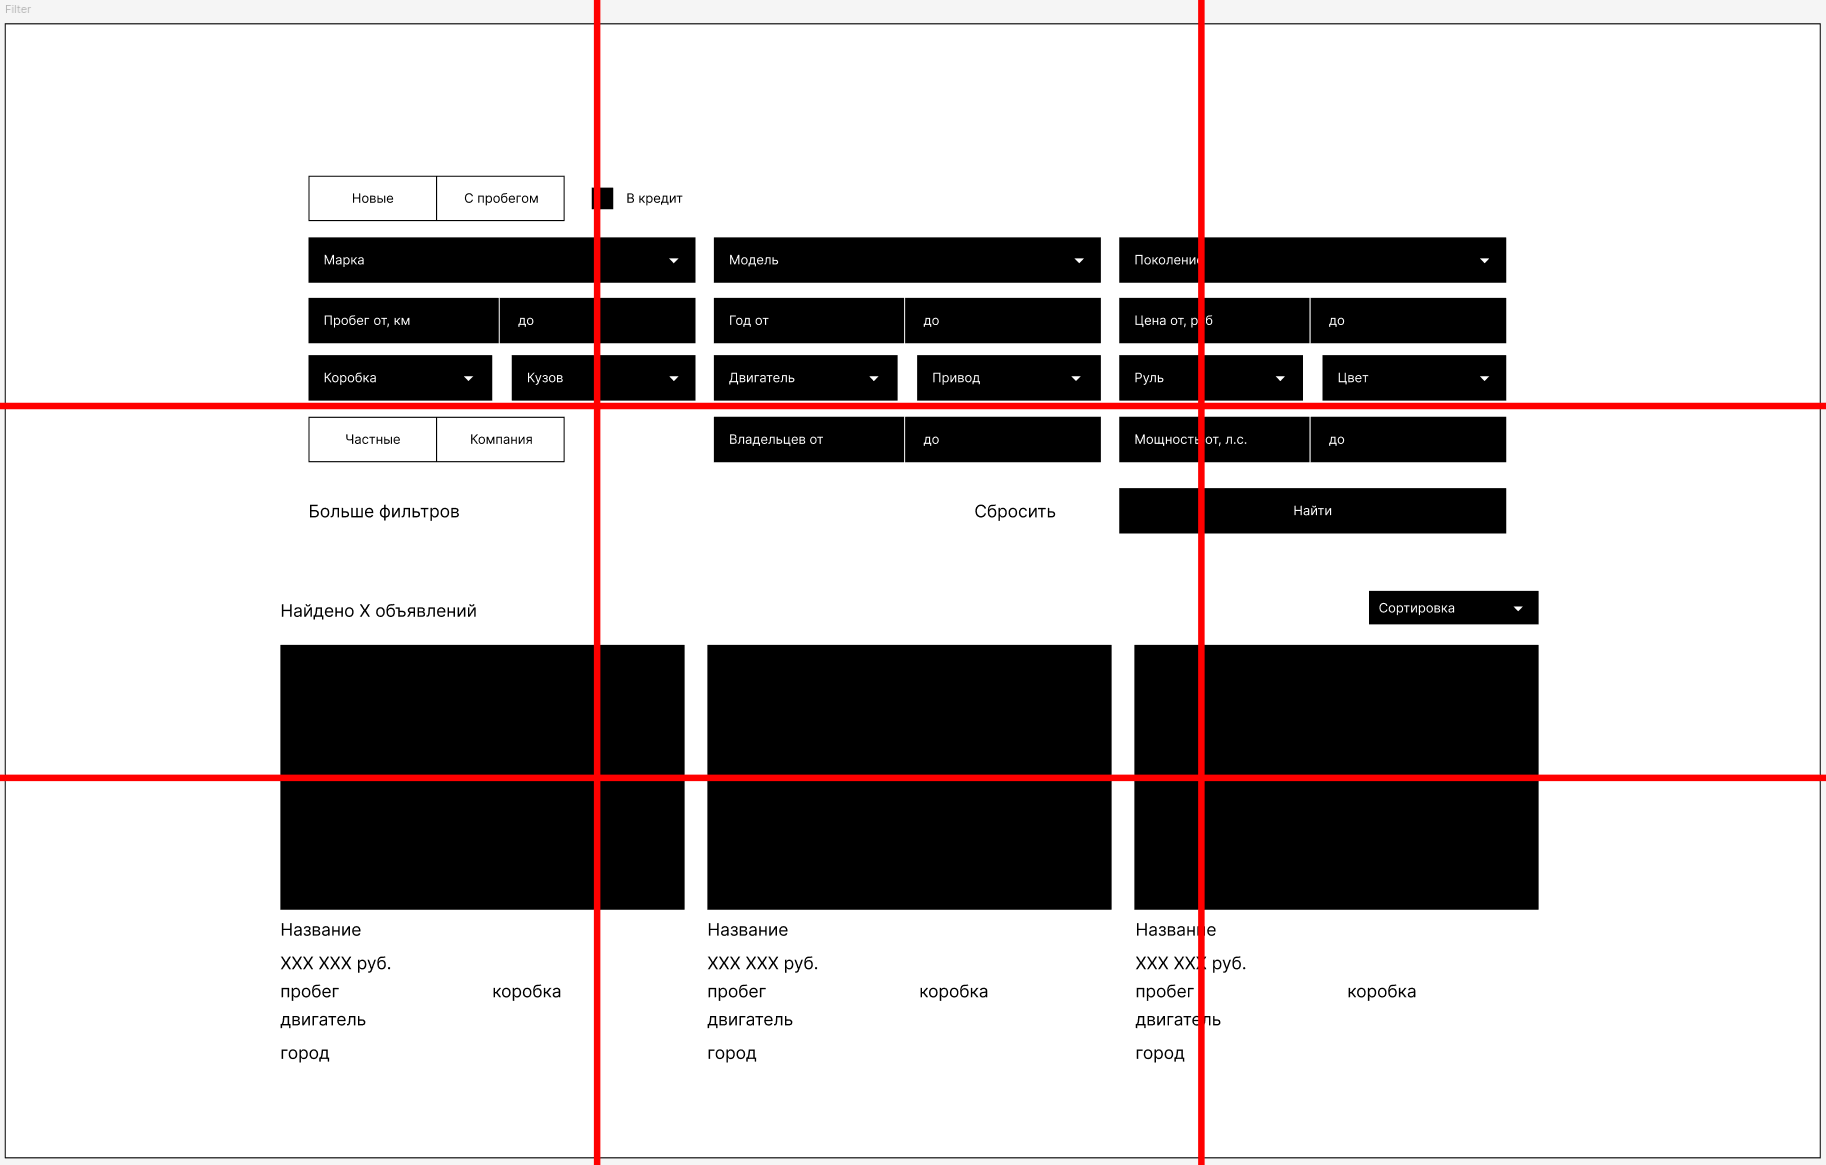
\includegraphics[width=\linewidth]{third_filter}}
    \captionof{figure}{Правило третей на странице поиска с фильтрами}
\end{minipage}
\bigskip

\noindent
\begin{minipage}{\linewidth}
    \fbox{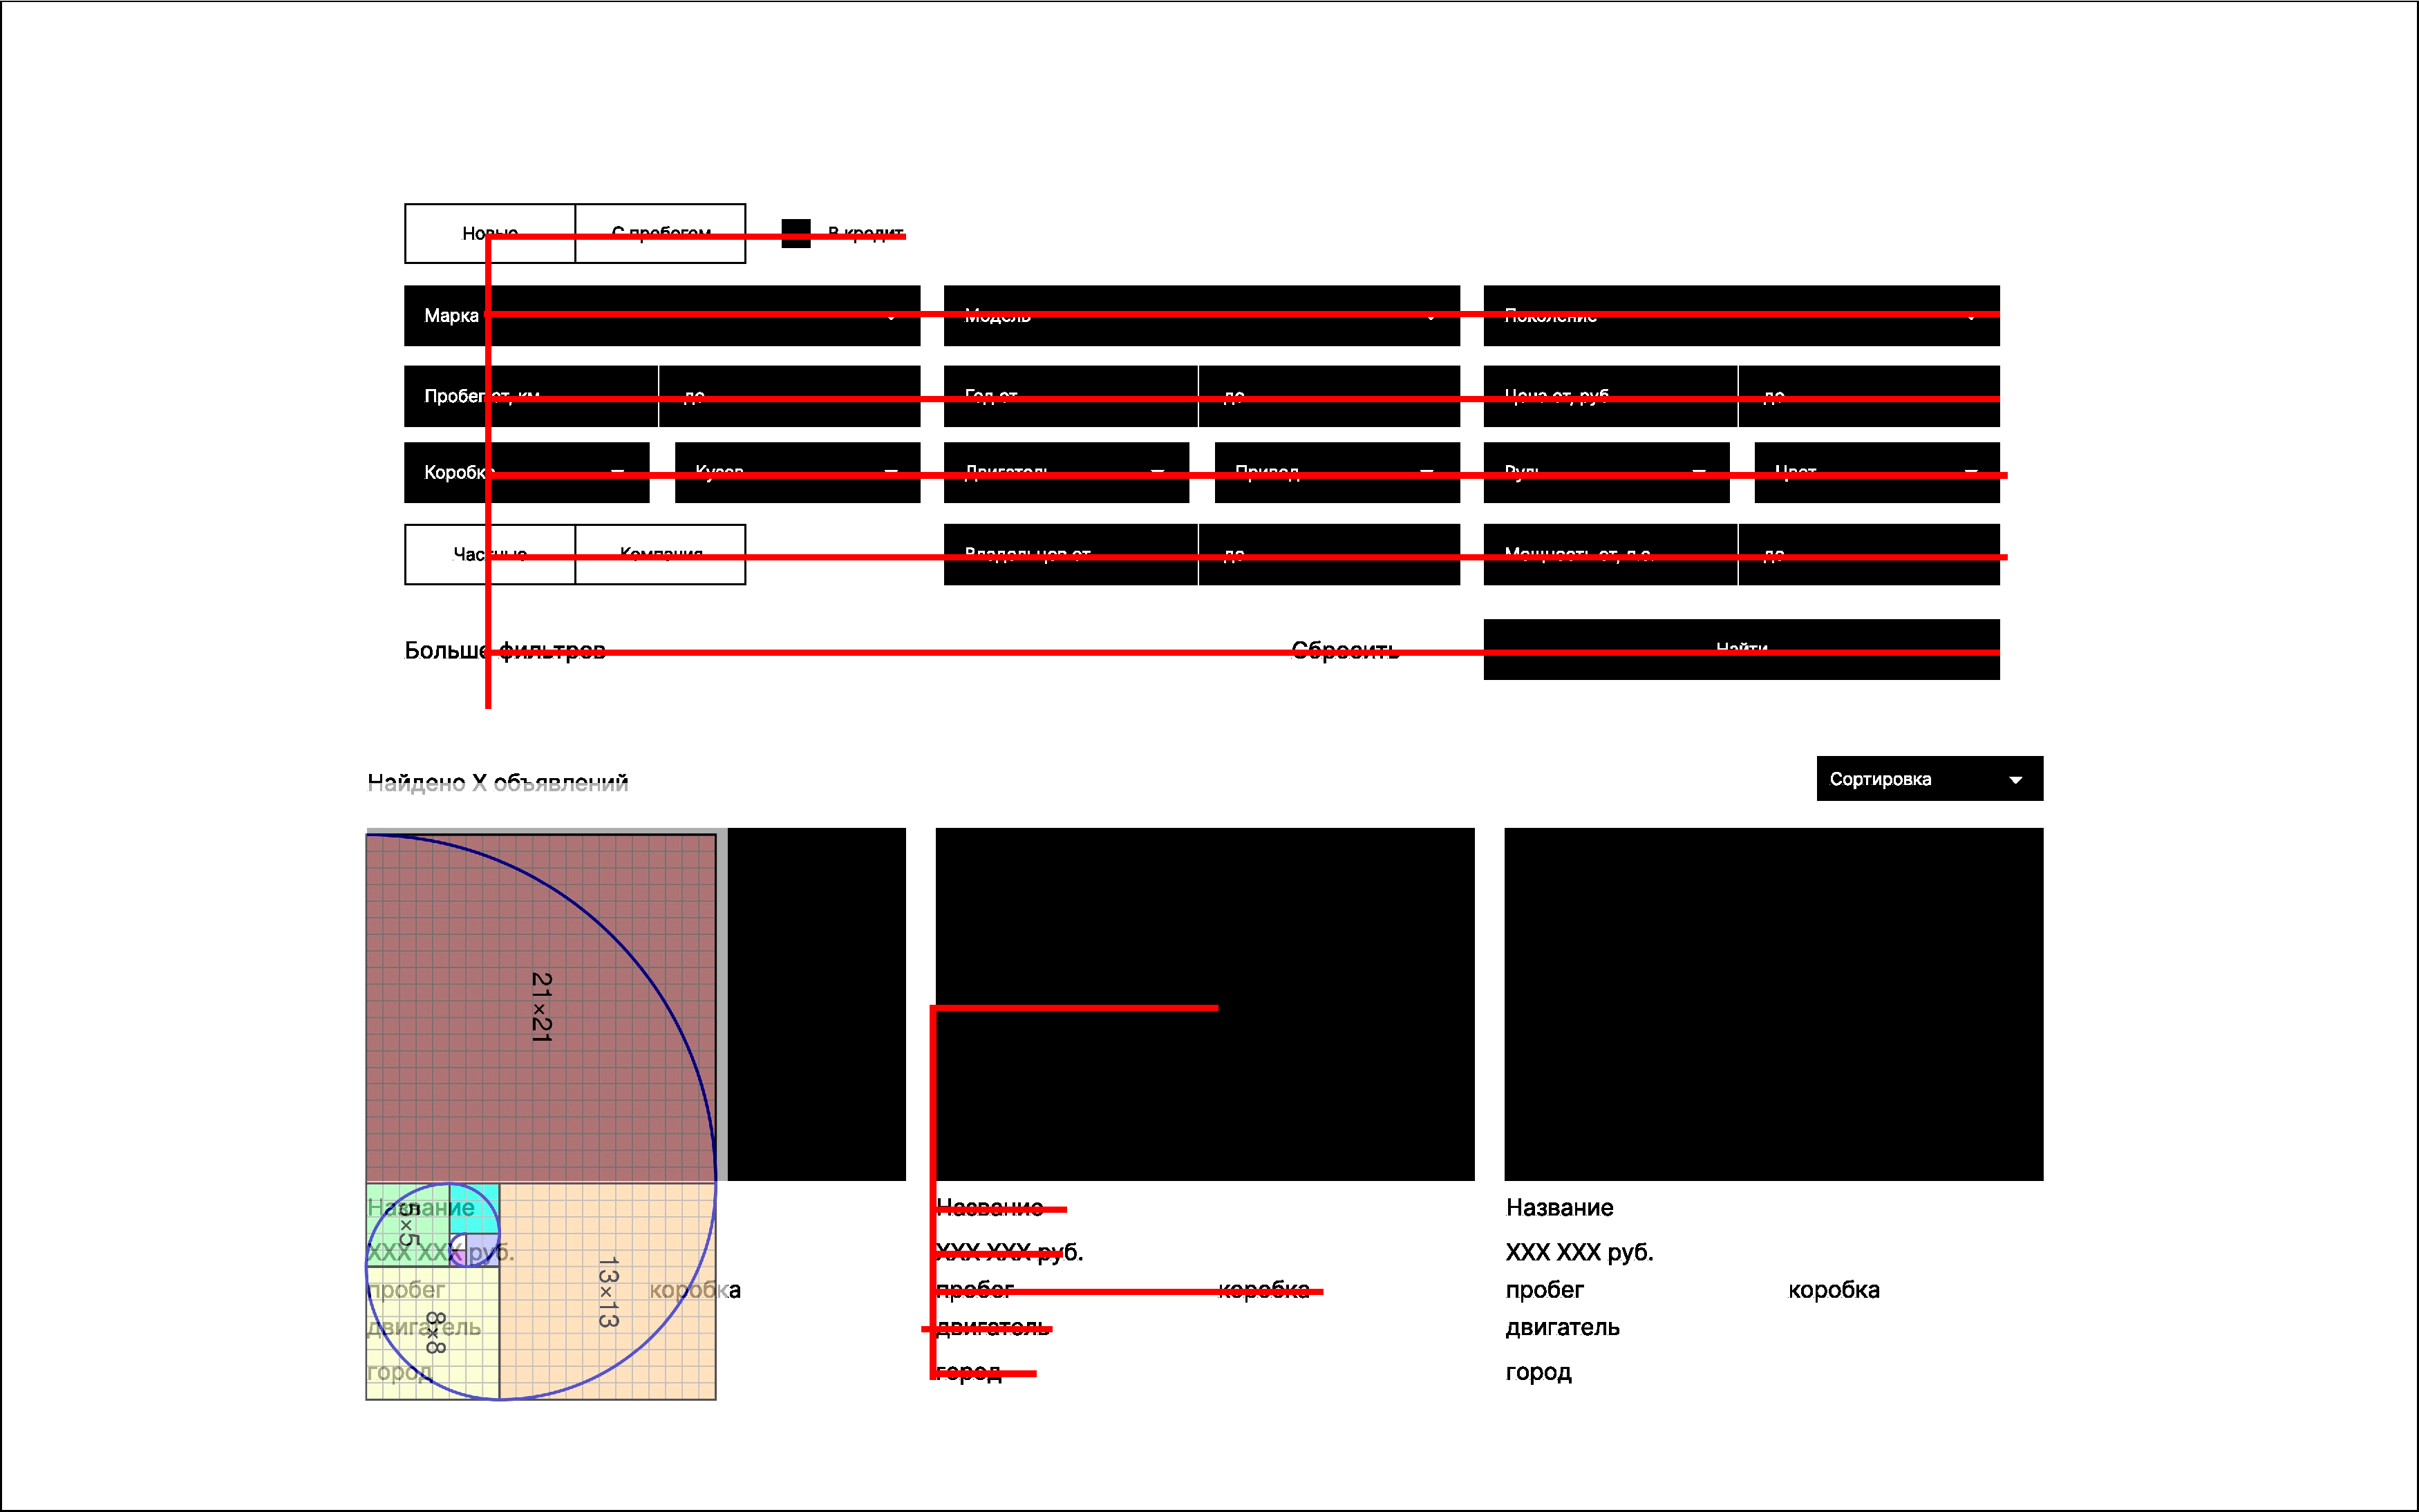
\includegraphics[width=\linewidth]{Filter-1}}
    \captionof{figure}{Правило третей и золотая спираль на странице поиска с фильтрами}
\end{minipage}
\bigskip

\noindent
\begin{minipage}{\linewidth}
    \fbox{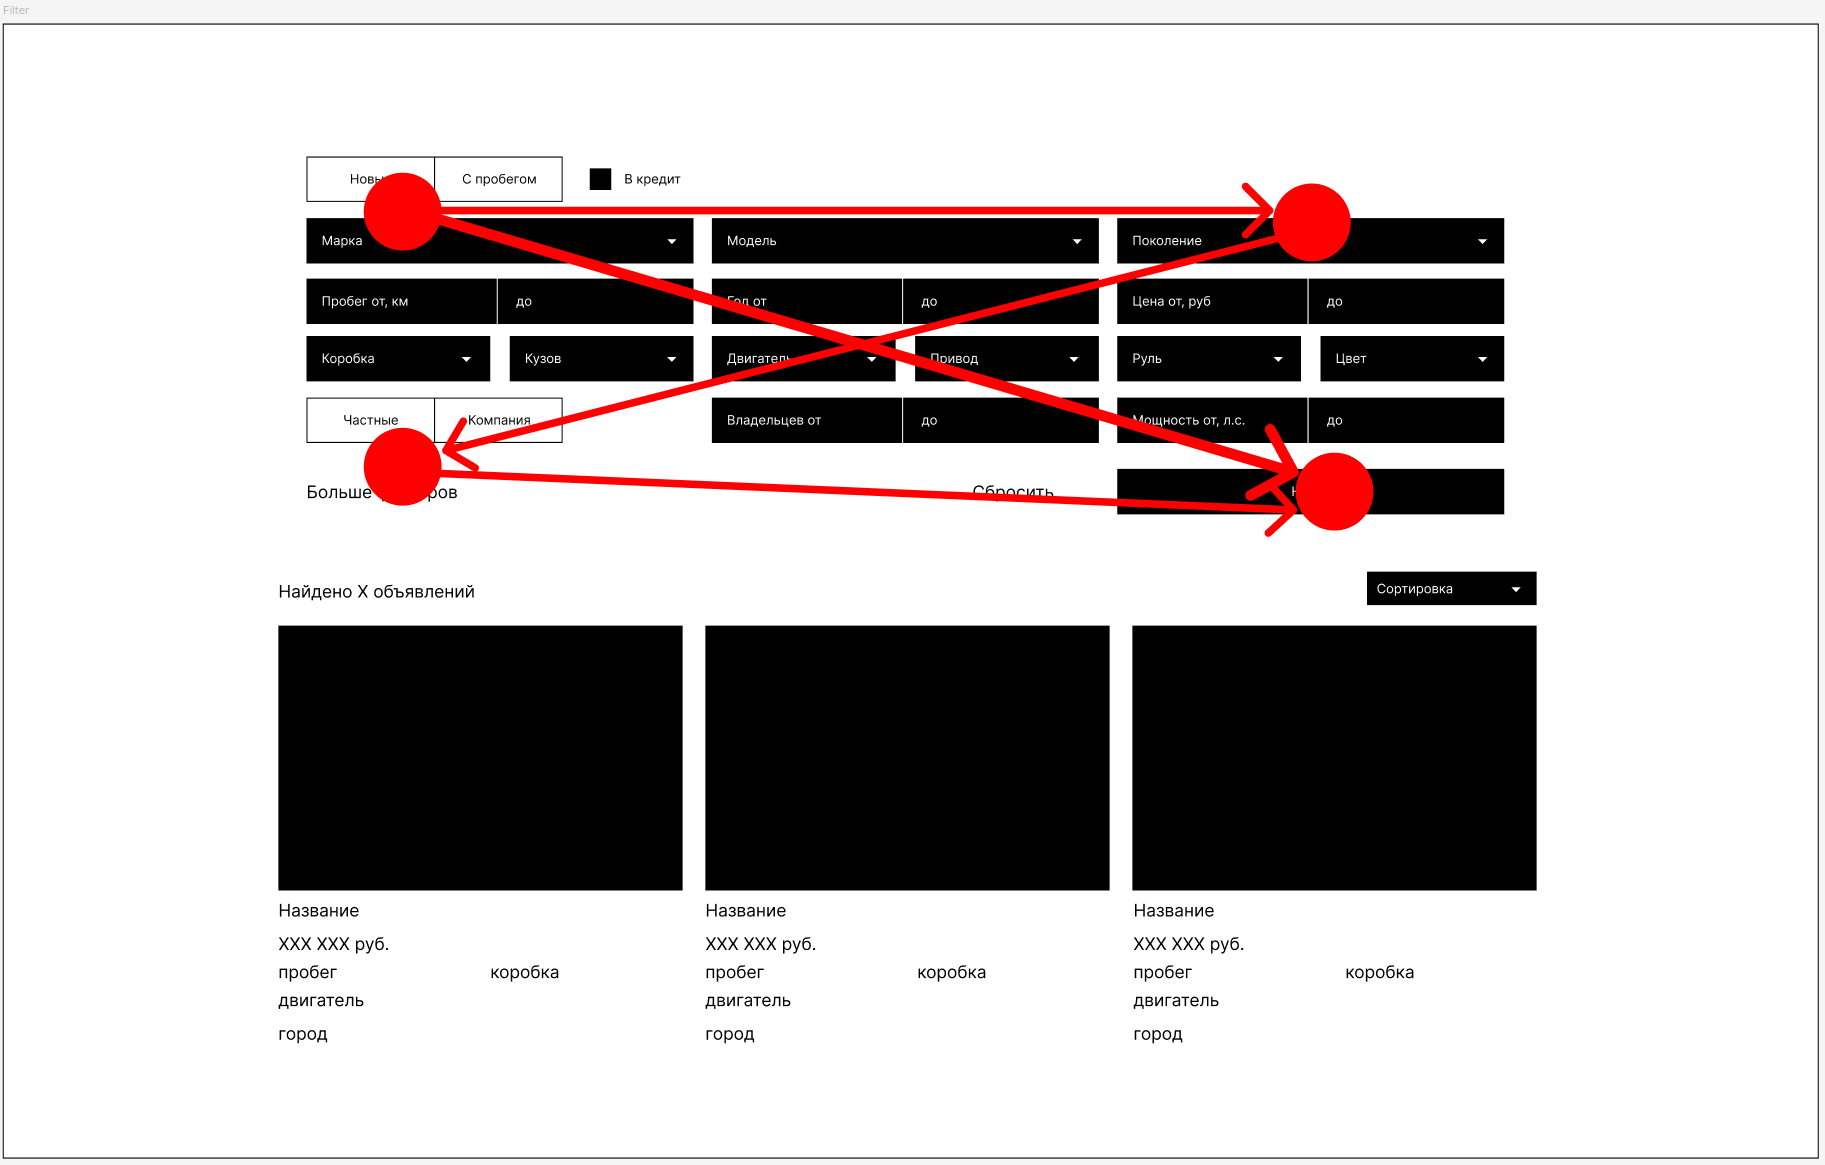
\includegraphics[width=\linewidth]{filter_f_gs}}
    \captionof{figure}{Диаграмма Гутенберга на странице поиска с фильтрами}
\end{minipage}
\bigskip

\noindent
\begin{minipage}{\linewidth}
    \fbox{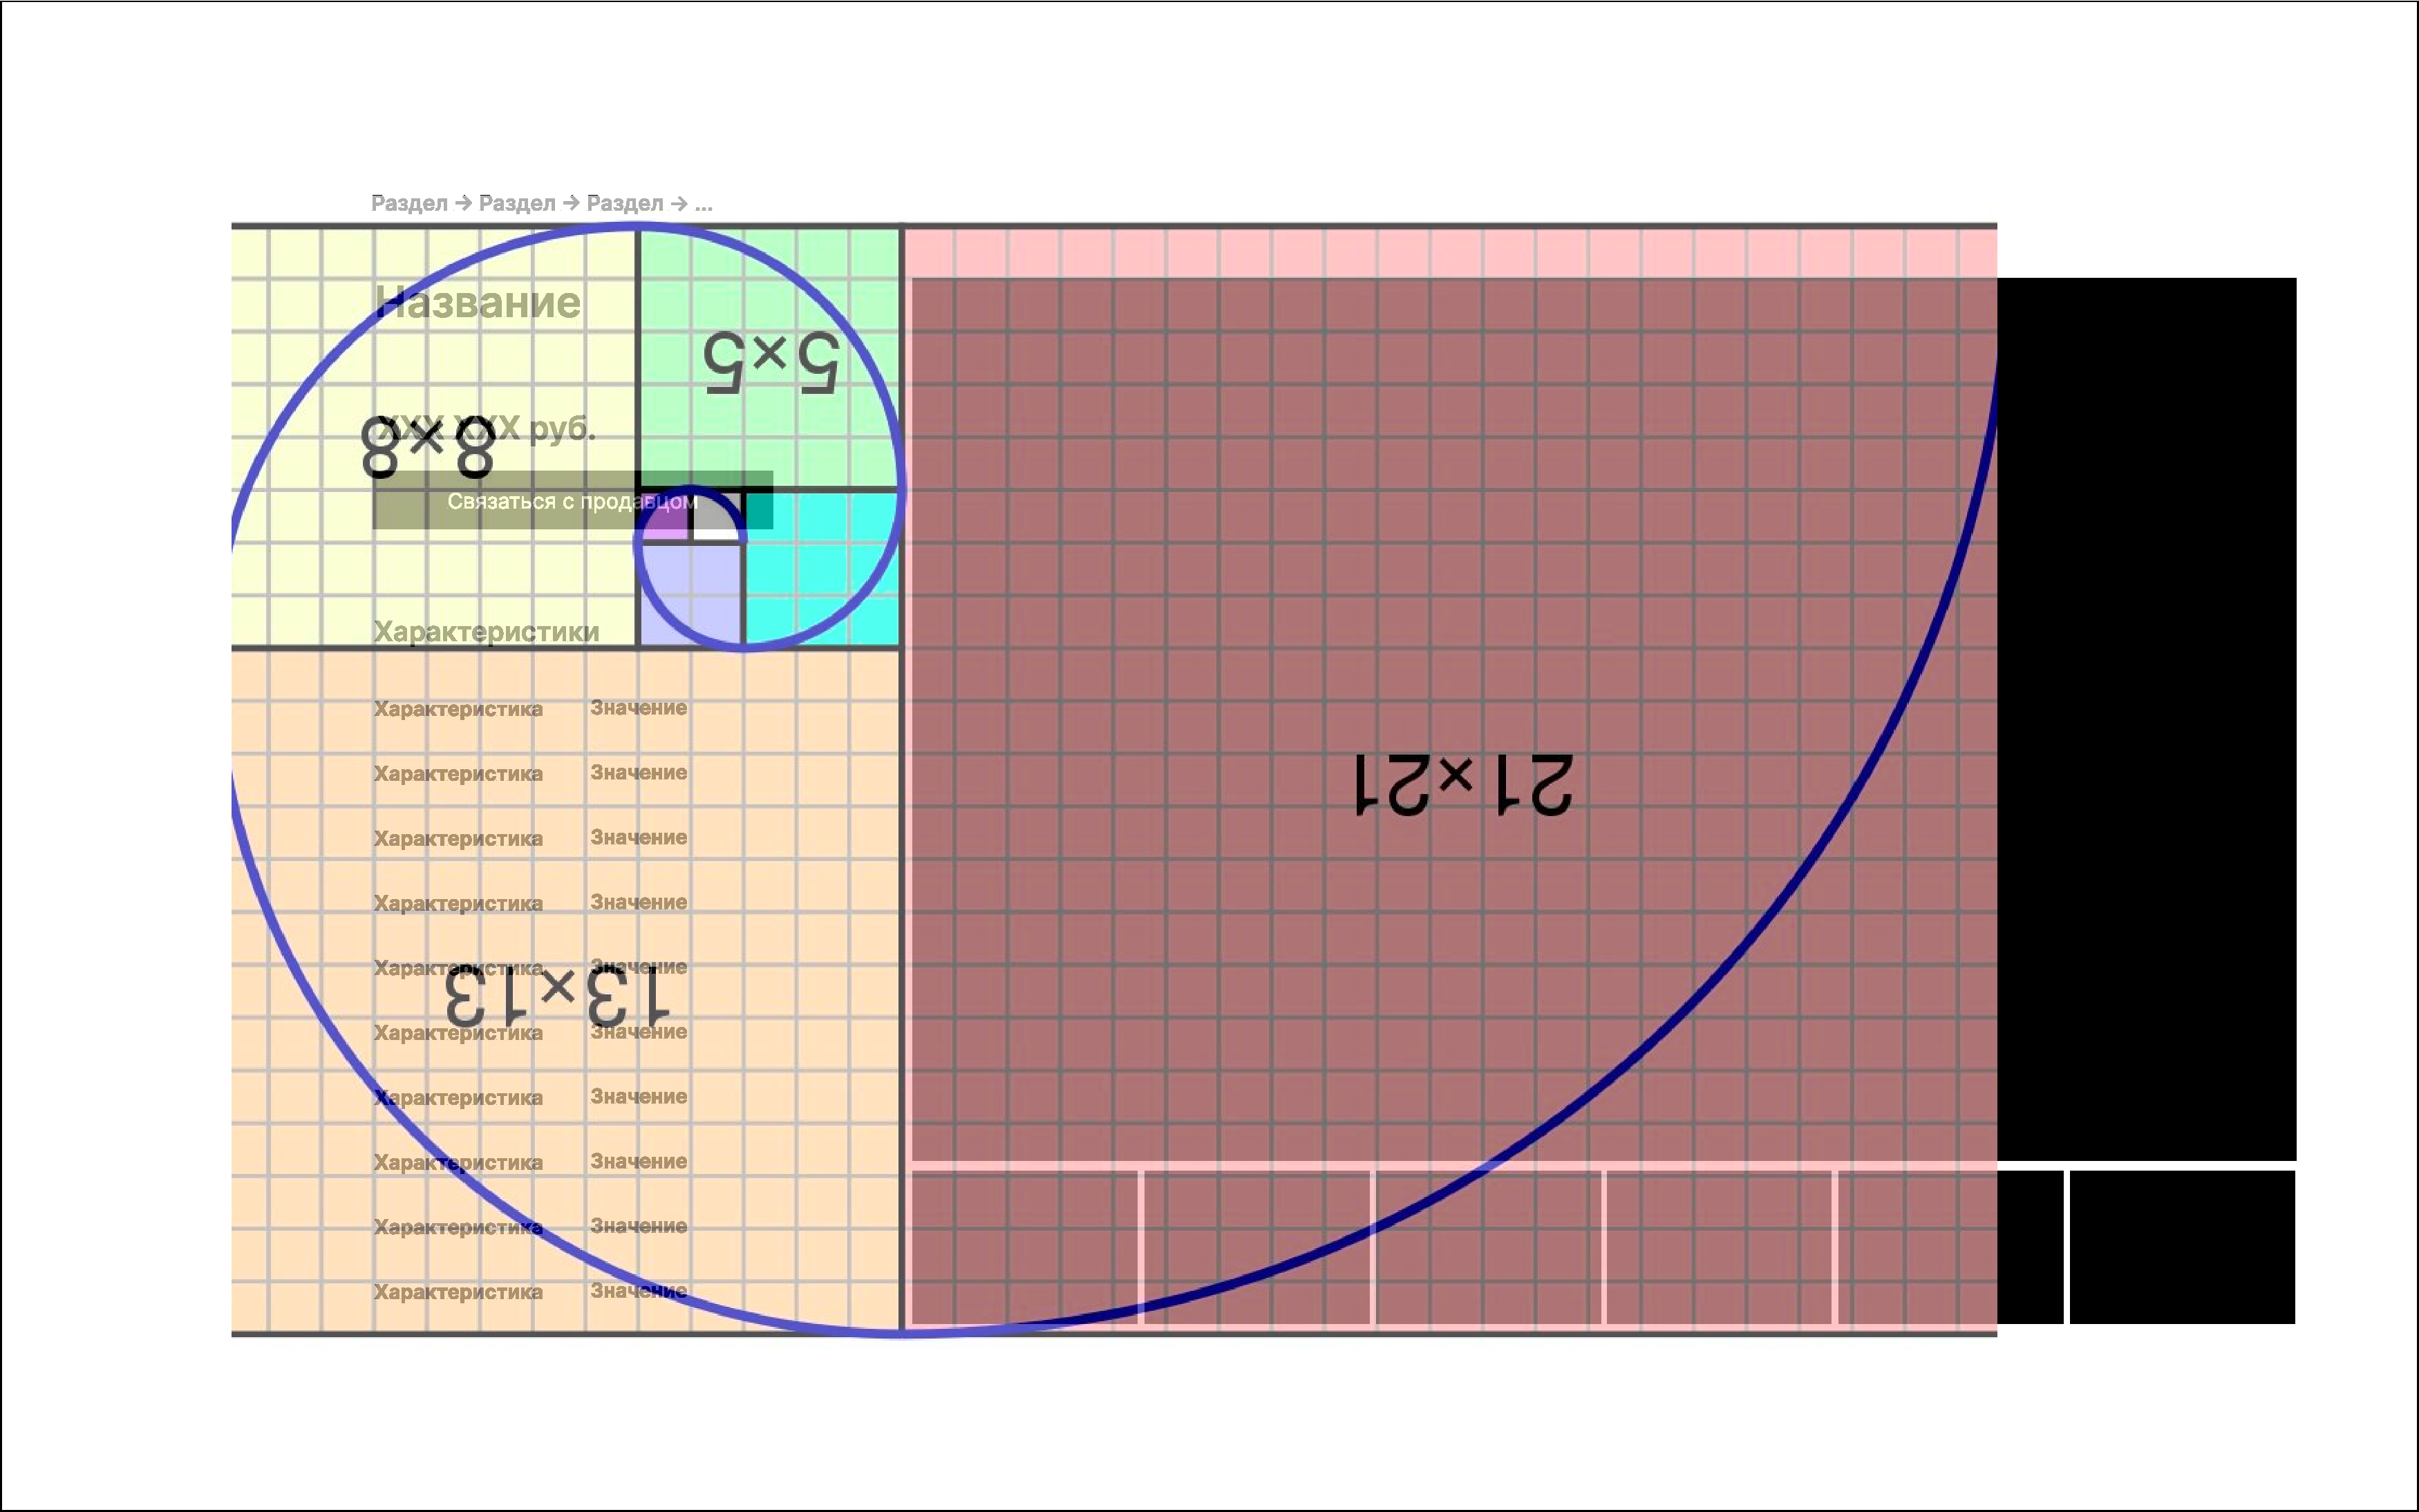
\includegraphics[width=\linewidth]{selected_spiral}}
    \captionof{figure}{Золотая спирать Фибоначчи на странице выбранного объявления}
\end{minipage}
\bigskip

\noindent
\begin{minipage}{\linewidth}
    \fbox{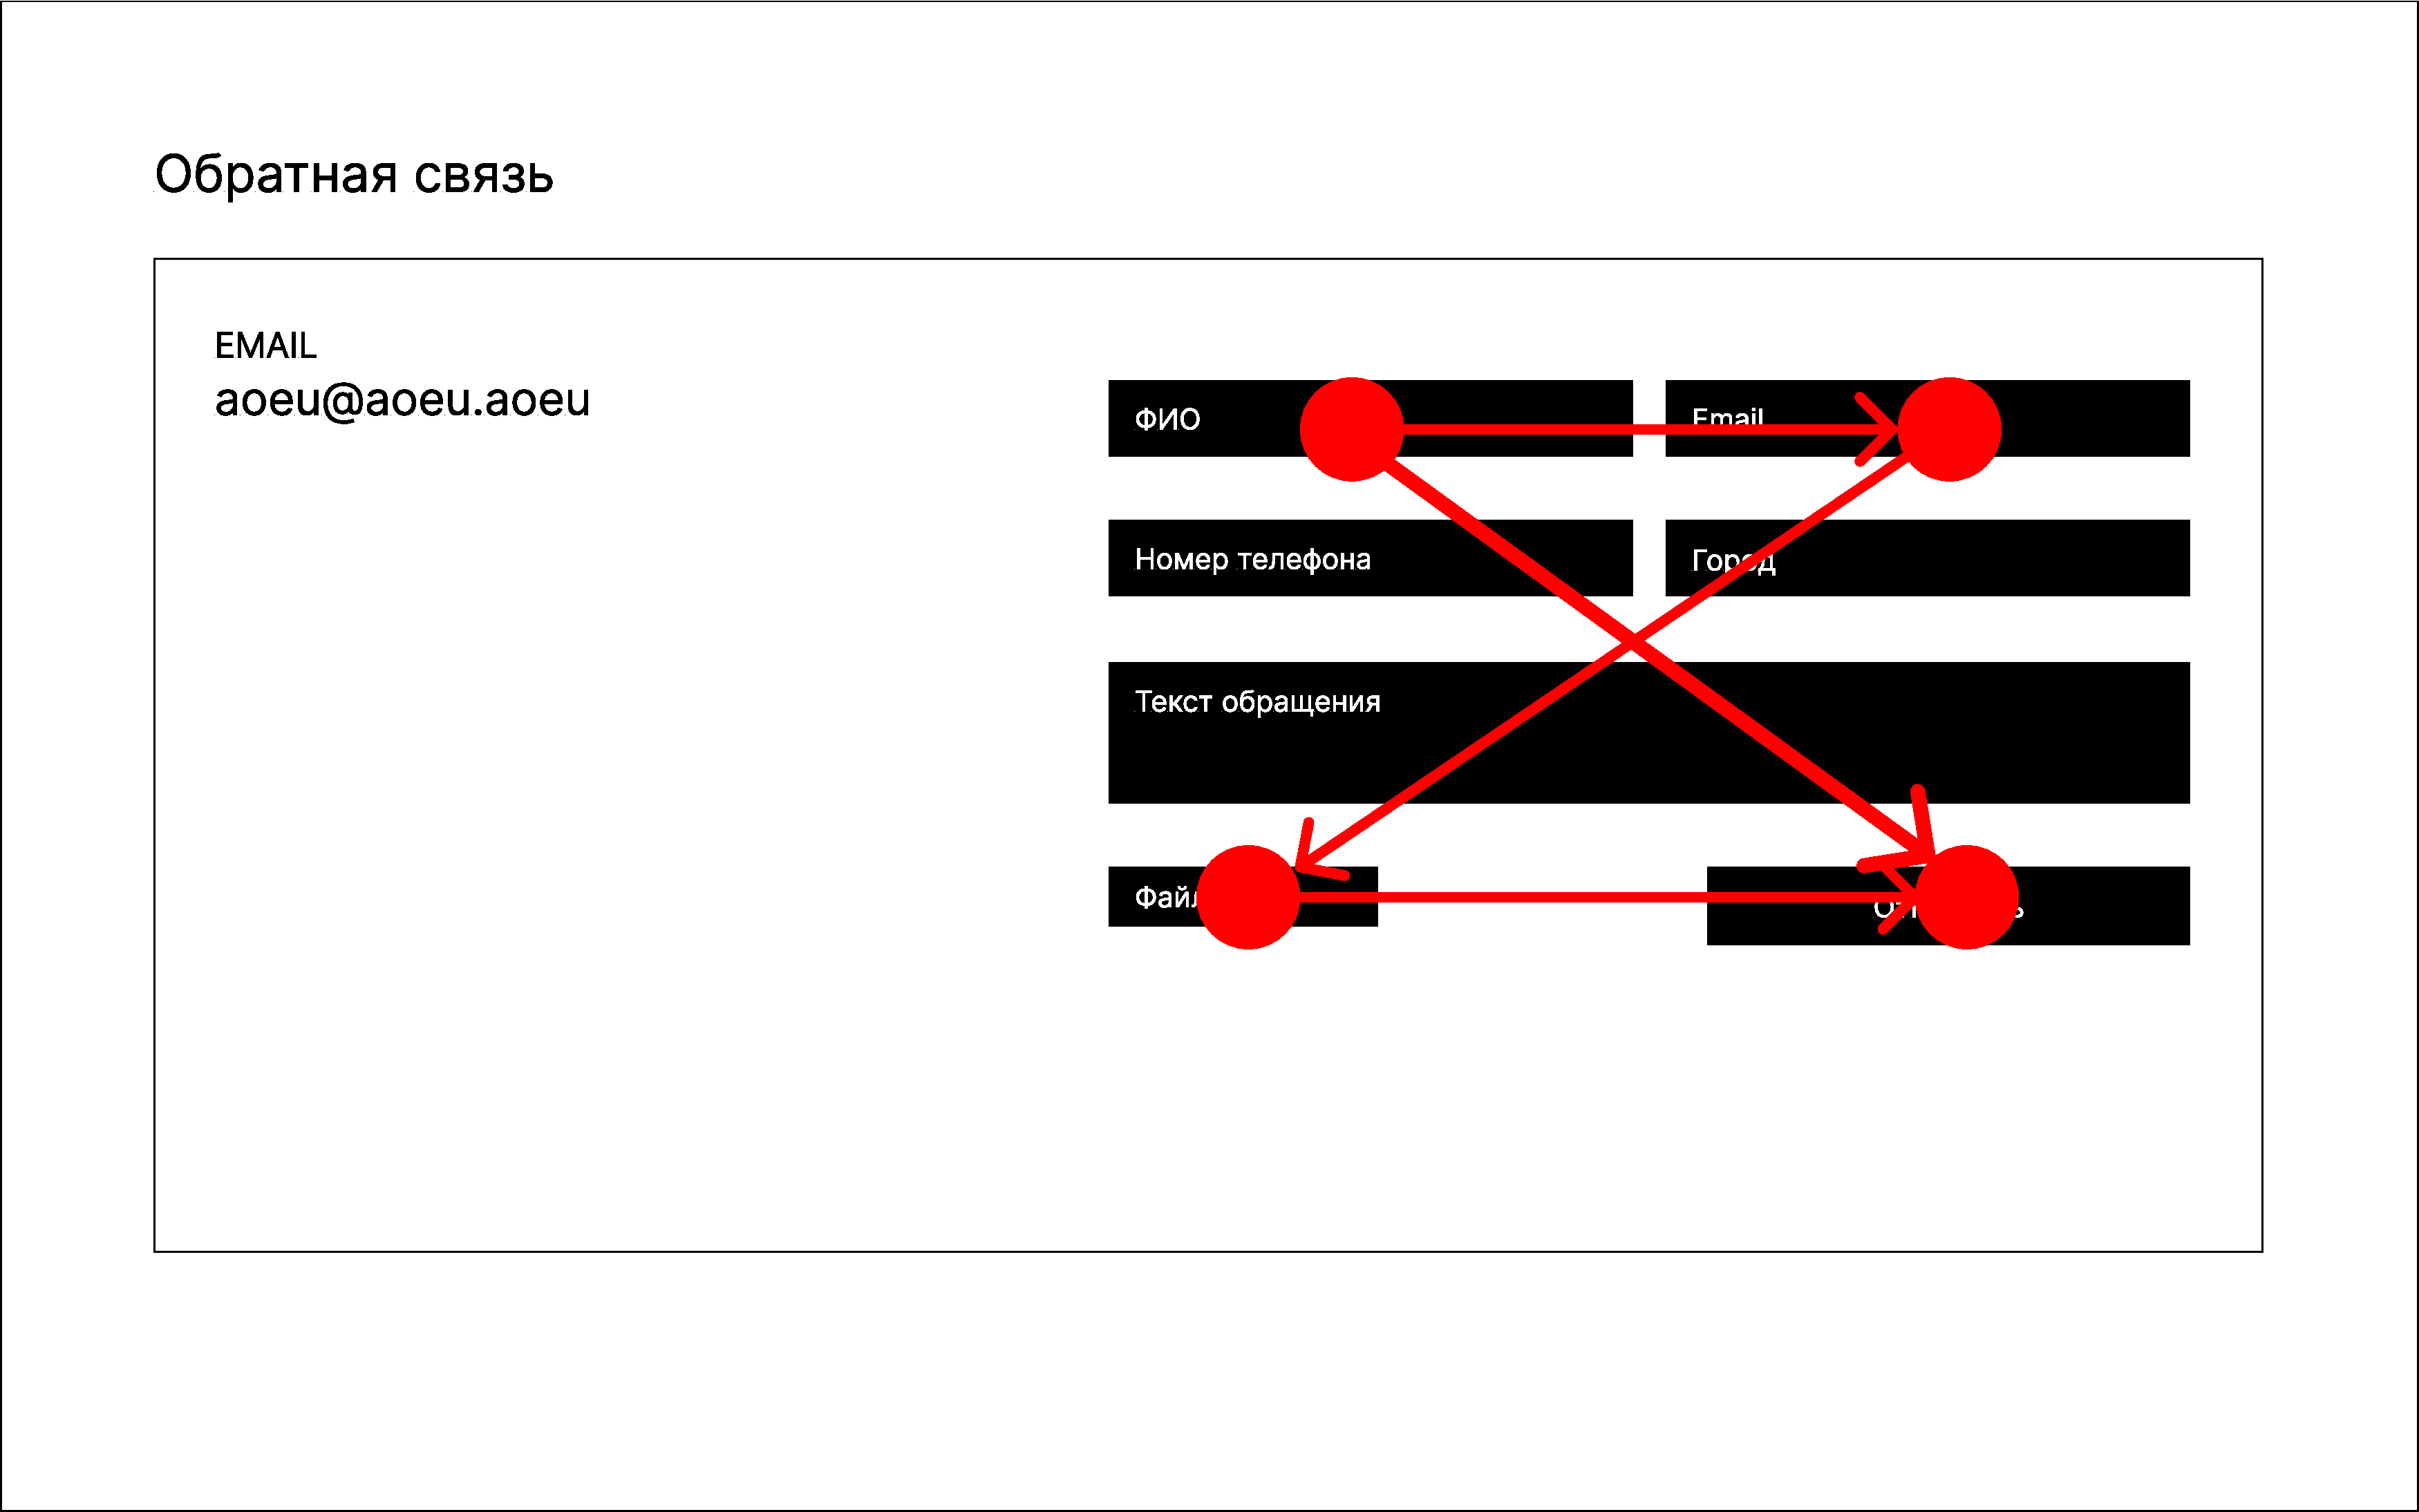
\includegraphics[width=\linewidth]{contacts_diag}}
    \captionof{figure}{Диаграмма Гутенберга на странице обратной связи}
\end{minipage}
\bigskip

\textbf{Контрольные вопросы и ответы}

\begin{enumerate}
    \item Что такое композиция? Основные понятия в композиции.

    Композиция – это процесс организации элементов в дизайне, создающий гармоничное и сбалансированное целое. Основные понятия композиции включают целесообразность, единство, равновесие, наличие смыслового центра и гармонию. Композиция обеспечивает логичное расположение частей для ясности и стройности формы, а также для восприятия содержания.

\item Основной закон композиции.

    Основной закон композиции гласит, что элементы дизайна должны быть организованы таким образом, чтобы создавать единое целое, где каждый элемент выполняет свою функцию. Это предполагает гармоничное восприятие и подчинение всех элементов общему смысловому и визуальному центру.

\item Какие средства гармонизации композиции вам известны? Дайте характеристику каждой. Пояснить, как они используются в проектировании интерфейса.

    \begin{itemize}
        \item Баланс - создаёт равновесие между элементами, которое может быть симметричным или асимметричным. В интерфейсе помогает создавать стабильные и гармоничные композиции.
        \item Пропорции - отношение размеров между элементами, например, с использованием «золотого сечения». Позволяет добиться гармонии и привлекательности в интерфейсе.
        \item Ритм - повторение элементов для создания движения. В интерфейсе помогает направлять взгляд пользователя.
        \item Контраст - использование элементов с разными свойствами для акцента. В интерфейсе контраст привлекает внимание к ключевым элементам.
        \item Цвет - создаёт гармонию и акценты, управляет эмоциональным восприятием интерфейса.
        \item Пространство - правильное распределение свободного пространства помогает организовать элементы интерфейса и выделить ключевые области.
    \end{itemize}

\item Что такое «фокальная точка», «правило третей», «золотое сечение» и "золотая спираль"? Как они применяются при проектировании дизайна интерфейса информационной системы?
    \begin{itemize}
        \item Фокальная точка – элемент, который привлекает основное внимание пользователя. Применяется для акцента на ключевых элементах интерфейса.
        \item Правило третей – деление области на три части для создания сбалансированного дизайна. Используется для расположения важных элементов в местах пересечения линий.
        \item Золотое сечение – математическое соотношение, формирующее гармонию (1:1.618). Применяется для пропорционального размещения элементов.
        \item Золотая спираль – основана на последовательности Фибоначчи и помогает размещать элементы по спирали, привлекая внимание к центру композиции.
    \end{itemize}

\item Принципы визуальной иерархии элементов интерфейса информационной системы.

    Принципы визуальной иерархии включают использование размера, контраста, цвета, пространства и расположения для выделения элементов. Например, крупные или контрастные элементы привлекают внимание, а правильное распределение пространства создаёт иерархию, помогая пользователю легче воспринимать информацию и находить нужные элементы.
\end{enumerate}

\end{document}
